      
               
                \begin{ledgroupsized}[r]{120mm}
                \footnotesize 
                \pstart                
                \noindent\textbf{\"{U}berlieferung:}   
                \pend
                \end{ledgroupsized}
            
              
                            \begin{ledgroupsized}[r]{114mm}
                            \footnotesize 
                            \pstart \parindent -6mm
                            \makebox[6mm][l]{\textit{L}}Reinschrift mit wenigen Korrekturen: LH XXXV 12, 1 Bl. 327. 1 Bl. 2\textsuperscript{o}. 2~S. R\"{a}nder durch Papierbad rekonstruiert. Bl. 327 r\textsuperscript{o} zweispaltig beschrieben, wobei die rechte Spaltenbreite 1/3 der linken Spaltenbreite betr\"{a}gt. Bl. 327 v\textsuperscript{o} enth\"{a}lt eine ganzseitige Zeichnung. Diese Zeichnung ist deutlich kleiner und um 90\textsuperscript{o} gedreht auch oben rechts auf Bl. 327 r\textsuperscript{o} aufgef\"{u}hrt.\\Cc 2, Nr. 1551 \pend
                            \end{ledgroupsized}
                %\normalsize
                \vspace*{5mm}
                \begin{ledgroup}
                \footnotesize 
                \pstart
            \noindent\footnotesize{\textbf{Datierungsgr\"{u}nde}: Im Rahmen der vielseitigen Anwendungsm\"{o}glichkeiten, die Leibniz f\"{u}r seine Maschine angibt, teilt er mit, sich \"{u}ber die Konstruktion eines motus quasi-perpetuus gesondert \"{a}ußern zu wollen. Die Ank\"{u}ndigung ist in der Handschrift LH XXXVII 5 Bl. 92\textendash 93 realisiert und wird in \textit{LSB} VIII, 2 abgedruckt. Das dort beschriebene Horologium ventaneum ist Teil der Auseinandersetzung Leibniz' mit dem Perpetuum mobile, die bereits 1671 zu einer eigenen Konstruktion (vgl. N. 60) f\"{u}hrt. Nach weiteren Versuchen formuliert Leibniz die Problem\-stellung neu. Er fragt nun danach, unter welchen Bedingungen \"{u}berhaupt eine konti\-nuierliche Bewegung m\"{o}glich ist (LH XXXVII 5 Bl. 57\textendash 59) und gibt daf\"{u}r eine Konstruktion an. Dieses Manuskript wurde von ihm selbst auf 1674 datiert. In einem n\"{a}chsten Schritt wird die Frage diskutiert, wie es gelingt, unter der Voraussetzung diskontinuierlicher Anregungen zu einer kontinuierlichen Bewegung zu gelangen. Die Antwort darauf ist die Konstruktion des erw\"{a}hnten Horologium ventaneum. Aus der Gedankenentwicklung und den dazu geh\"{o}rigen Konstruktionen ergibt sich, dass die Idee einer Winduhr erst nach dem Manuskript von 1674 entstanden sein kann. Darauf beruht die Datierung.}
                \pend
                \end{ledgroup}
            
                \vspace*{8mm}
                %\newpage
                \pstart 
                \normalsize
            \centering{[327~r\textsuperscript{o}] \textso{Machina Progressionum }\protect\index{Sachverzeichnis}{machina!progressionum}\edtext{}{\lemma{\textso{Machina Progressionum}}\Afootnote{\textit{doppelt unterstrichen}}}\\ in qua motus tardissimus et celerrimus\\ viresque maximae et minimae, quousque materia\\ permittit, ostendi possunt.} \pend \vspace{1.0ex}
            \pstart Sunto Trochleae\protect\index{Sachverzeichnis}{trochlea} quotcunque sibi aequales, magnitudinis datae; \textit{a, b, c, d, e, f} cuilibet earum praeter primam \textit{a} implantata sit alia Trochlea\protect\index{Sachverzeichnis}{trochlea} eminens concentrica \textit{g, h, i, k, l} \edtext{cujus circumferentia}{\lemma{\textit{g, h, i, k, l}}\Afootnote{ \textit{ (1) }\ quae \textit{ (2) }\ cujus circumferentia \textit{ L}}} sit decima pars majoris. Conjugantur Trochleae\protect\index{Sachverzeichnis}{trochlea} chordis eum in modum, ut eadem chorda applicetur circumferentiae praecedentis majoris \textit{a} et circumferentiae sequentis minoris \textit{g} similiter \textit{b} et \textit{h} item \textit{c} et \textit{k} item \textit{e} et \textit{l}. Haec jam constructio est.\pend
              \vspace{1.0ex}
              \begin{center}
              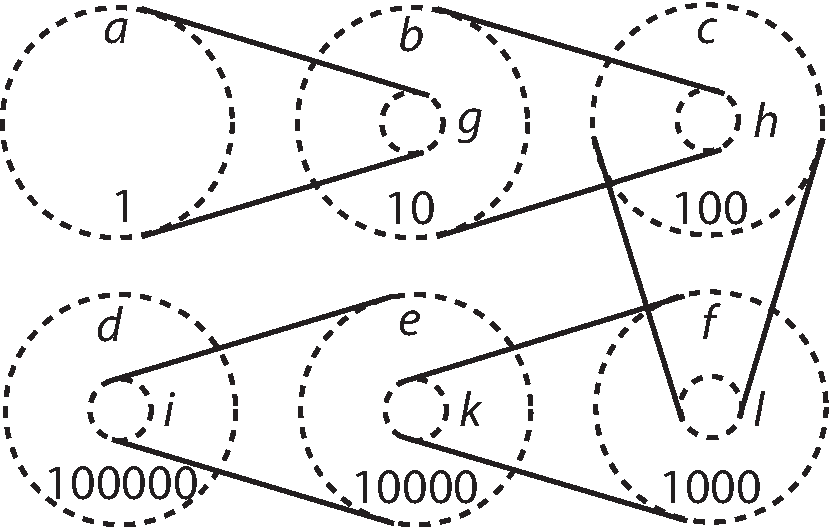
\includegraphics[width=0.35\textwidth]{images/35_12_1_327r}
              \vspace{0.5ex}
              \\\textit{[Fig. 1]}
              \end{center}
            \pstart 
            \begin{center}\textso{Motus celerrimus} in hac Machina ita producetur.\end{center}\pend \vspace{1.0ex} \pstart  Circumage Trochleam\protect\index{Sachverzeichnis}{trochlea} majorem primam \textit{a} semel. Eodem tempore circumagetur trochlea\protect\index{Sachverzeichnis}{trochlea} minor \textit{g} decies, quare et \edtext{Trochlea}{\lemma{et}\Afootnote{ \textit{ (1) }\ chorda \textit{ (2) }\ Trochlea \textit{ L}}} \textit{b}. Ergo Trochlea\protect\index{Sachverzeichnis}{trochlea} minor \textit{h} cum sua majore \textit{c} centies et \textit{i} cum sua majore \textit{d} millies, et \textit{k} cum \textit{e} decies millies; et \textit{l} cum \textit{f} centies millies. Ergo quo tempore Trochlea\protect\index{Sachverzeichnis}{trochlea} \textit{a} circumagitur semel, circumagetur Trochlea\protect\index{Sachverzeichnis}{trochlea} \textit{f} ei aequalis centies millies. Pone circumactionem Trochleae\protect\index{Sachverzeichnis}{trochlea} \textit{a} esse celeritatis ordinariae, erit circumactio Trochleae\protect\index{Sachverzeichnis}{trochlea} \textit{f} centies millies ordinaria major. Si plures Trochleae\protect\index{Sachverzeichnis}{trochlea} esse supponantur erit motus millies millies. Idque continuari potest, quousque Machinae sunt capaces. \edtext{Erit ergo Machina [Progressionum]\edtext{}{\Afootnote{Proportionum\textit{\ L \"{a}ndert Hrsg. } }}\protect\index{Sachverzeichnis}{machina!progressionum} ipsa Cochlea\protect\index{Sachverzeichnis}{cochlea} efficacior.}{\lemma{}\Afootnote{Erit ergo Machina [Progressionum]\edtext{}{\Afootnote{Proportionum\textit{\ L \"{a}ndert Hrsg. } }}\protect\index{Sachverzeichnis}{machina!progressionum} ipsa Cochlea\protect\index{Sachverzeichnis}{cochlea} efficacior. \textit{ erg.} \textit{ L}}}\pend \pstart  At \textso{Motus tardissimus} fiet, inverso modo. Nimirum si circumagatur Trochlea\protect\index{Sachverzeichnis}{trochlea} \edtext{ultima}{\lemma{}\Afootnote{ultima \textit{ erg.} \textit{ L}}} \textit{f} semel, motu ordinario; eodem tempore Trochleae\protect\index{Sachverzeichnis}{trochlea} primae \textit{a} non nisi pars centesima millesima circumagetur. Erit ergo motus ejus centies millies ordinario tardior, tametsi continuus.\pend \pstart Ergo \textso{vires quantaecunque minimae erunt,} si applicentur Trochleae\protect\index{Sachverzeichnis}{trochlea} primae, et \textso{vires quantulaecunque maximae erunt,} si applicentur Trochleae\protect\index{Sachverzeichnis}{trochlea} ultimae. Cum enim potentia fiat ex ductu gravitatis\protect\index{Sachverzeichnis}{gravitas} (alteriusve potentiae absolutae) in celeritatem, manifestum est, id quod centies millies levius est alio, posse ei aequiponderare, si grave Trochleae\protect\index{Sachverzeichnis}{trochlea} primae, leve ultimae applicetur. \pend \vspace{2.0ex} \pstart \centering Objectiones seu difficultates.\pend \vspace{1.0ex} \pstart Objicietur Trochleam\protect\index{Sachverzeichnis}{trochlea} primam non nisi maxima difficultate circumactum iri. Postremas enim etsi ex materia levissima supponerentur, millies, decies millies, centies millies, amplius quam ante ponderaturas, et atomum quantulamcunque  postremae Trochleae\protect\index{Sachverzeichnis}{trochlea} impositam magni ponderis\protect\index{Sachverzeichnis}{pondus} fore; ac proinde aerem ipsum ejus motui fortissime obstiturum.\pend \pstart Responderi, potest, \textso{primo} hanc objectionem esse tantum contra motum celerrimum viresque Trochleae\protect\index{Sachverzeichnis}{trochlea} primae applicatas; non contra tardissimum viresque ultima appensas. \textso{Deinde} non desunt nobis vires maximae, si modo recte applicentur, quales sunt pulveris Pyrii\protect\index{Sachverzeichnis}{pulvis!pyrius}, Aerisque compressi aut distracti. Circumagatur ergo Trochlea\protect\index{Sachverzeichnis}{trochlea} prima aliquousque, pulvere pyrio\protect\index{Sachverzeichnis}{pulvis!pyrius} applicato; necesse erit, aut omnia rumpi, aut ultimam eodem tempore centies millies circumagi. Si repetenda saepius circumactio est, ac pulvis pyrius\protect\index{Sachverzeichnis}{pulvis!pyrius} sumtuosior videtur; aere idem propemodum effici potest.\pend \pstart  Objicietur ergo potius omnia ruptum iri. Fateor, si nimium continuetur haec decadica progressio: at stari potest intra mediocritatem, quousque scilicet Rotae chalybeae fortissimae, et chordarum loco catenae ferreae, impetum perferre possunt. Ac ne ob celeritatem motus chorda seu Catena Trochleam\protect\index{Sachverzeichnis}{trochlea} deserat, solaque moveatur, impediri potest, si in Trochleae\protect\index{Sachverzeichnis}{trochlea} circumferentia sint eminentiolae sive dentes, annulis catenae respondentes atque inter movendum interserti. \pend \vspace{2.0ex} \pstart \centering Usus Machinae Progressionum\protect\index{Sachverzeichnis}{machina!progressionum} \pend \vspace{1.0ex} \pstart Hi sunt multi, eorumque nonnulli plane admirandi. \pend \pstart (1) Motus tardissimi usus esse \edtext{potest}{\lemma{}\Afootnote{potest \textit{ erg.} \textit{ L}}} ad construendum Motum \edtext{quasi-perpetuum,}{\lemma{}\Afootnote{quasi-perpetuum,  \textbar\ eumque nihilominus regularem, \textit{ gestr.}\ \textbar\ quem \textit{ L}}}\protect\index{Sachverzeichnis}{motus!quasi-perpetuus} quem naturalis causa (ut Ventus) \edtext{suo}{\lemma{}\Afootnote{suo \textit{ erg.} \textit{ L}}} initio restituat, antequam totus decurrerit; de quo quia operae pretium videtur, separatim dicam.\pend \pstart (2) Motus celerrimi usus esse potest ad novi generis Molendina\protect\index{Sachverzeichnis}{molendinum} virium admirandarum construenda. Quae corpora crassa fortissime comminuant, quae corpora durissima efficacissime, secent tornentve. \edtext{Applicari Balisticis\protect\index{Sachverzeichnis}{balistica} ad corpora fortius projicienda (quod utile figuris conicis tornandis).}{\lemma{}\Afootnote{Applicari [...] tornandis). \textit{ erg.} \textit{ L}}} Quae idem intra nictum oculi millies agant atque ita tantundem efficiant tempore exiguo, quantum 100 aliae machinae hominesve longo. Poterunt etiam hac machina Experimenta physica innumera hactenus intentata suscipi; sunt enim quidam innumerabilium Experimentorum velut fontes, ut Thermometrum sive Fluddi\protect\index{Sachverzeichnis}{Thermometrum!Fluddi} sive Drebelii\protect\index{Sachverzeichnis}{Thermometrum!Drebelii}; perspicilla \protect\index{Sachverzeichnis}{perspecilla} sive Metii\protect\index{Namensregister}{\textso{Metius} ca. 1571\textendash 1628} sive Johannidae\protect\index{Sachverzeichnis}{Thermometrum!Iohannidae}; Recipiens Gerickii\protect\index{Sachverzeichnis}{Recipiens!Gerickii}; speculum Villettae\protect\index{Sachverzeichnis}{speculum!Villettae}\protect\index{Namensregister}{\textso{Drebbel} (Drebelius, Drebel), Fran\c{c}ois 1621\textendash 1698}, quibus unis institui possunt applicationes innumerabiles; ita ausim dicere, hanc \edtext{quoque}{\lemma{}\Afootnote{quoque \textit{ erg.} \textit{ L}}} Machinam multorum Experimentorum parentem fore. Constat enim omnes alterationes in natura fieri \textso{motu} quodam \textso{celerrimo insensibili.} Quare dubium nullum est \textso{Motu} quoque \textso{celerrimo sensibili} nova phaenomena plurima detectum iri. Constat motu produci calorem\protect\index{Sachverzeichnis}{calor}, apparebit ergo, quanto motu, quis caloris\protect\index{Sachverzeichnis}{calor} gradus, in quae corpora. An aquae, an aeri \edtext{ipsi}{\lemma{aeri}\Afootnote{ \textit{ (1) }\ ipse \textit{ (2) }\ ipsi \textit{ L}}} calor\protect\index{Sachverzeichnis}{calor} sensibilis imprimi hac ratione possit. Tam an corpora possint misceri, subigi, ad fermentationem\protect\index{Sachverzeichnis}{fermentatio} unionemque deduci; vicissim an separari, influxum redigi praecipitari. Compertum est pulverem plumbeum\protect\index{Sachverzeichnis}{pulvis!plumbeus} qui in Horologio arenario\protect\index{Sachverzeichnis}{horologium!arenarium} assidue versato diu mansit, alias plane a plumbo\protect\index{Sachverzeichnis}{plumbum} communi qualitates acquisivisse, ac difficulter fundi. Relatum mihi est a celebri quodam Medico, in Austria\protect\index{Ortsregister}{Osterreich@\"{O}sterreich (Austria)} Graecum nescio quem, auri bracteolas molae exiguae versatili incredibilis velocitatis, imposuisse; aurum\protect\index{Sachverzeichnis}{aurum} in massam quandam fluidam Mercurio\protect\index{Sachverzeichnis}{mercurius} currenti similem abiisse, ac demum continuato motu, in pulverem rubicundum concidisse. Hujus narrationes etsi fidem penes autorem esse velim, constat tamen \edtext{motu}{\lemma{tamen}\Afootnote{ \textit{ (1) }\ corpora \textit{ (2) }\ motu \textit{ L}}} celerrimo quantum humanae vires machinaeque assequi possunt, magnas in corporibus mutationes productum iri.\pend \pstart (3.) \textso{Motus celerrimi tardissimique simul,} ut scilicet vires celeriter onus tarde levetur; usus erit ad maximas moles elevandas, viribus minimis. Tarde fateor. Sed hoc saepe nihil refert. Si tamen celeritate opus est, poterunt virium loco machinae Aereae, aut pulvis pyrius\protect\index{Sachverzeichnis}{pulvis!pyrius}, aut animalia plura adhiberi. Quare non dubitem \textso{maximas rupes ope instrumenti hujus diffringi posse.} Quo casu Rotae dentatae\protect\index{Sachverzeichnis}{rota!dentata} omissis Trochleis\protect\index{Sachverzeichnis}{trochlea}, eadem proportione sibi rectius inserentur.\pend